\section{Discussion and Outlook (1 page)}
\label{sec:discussion_outlook}
\begin{figure}[t]
\centering
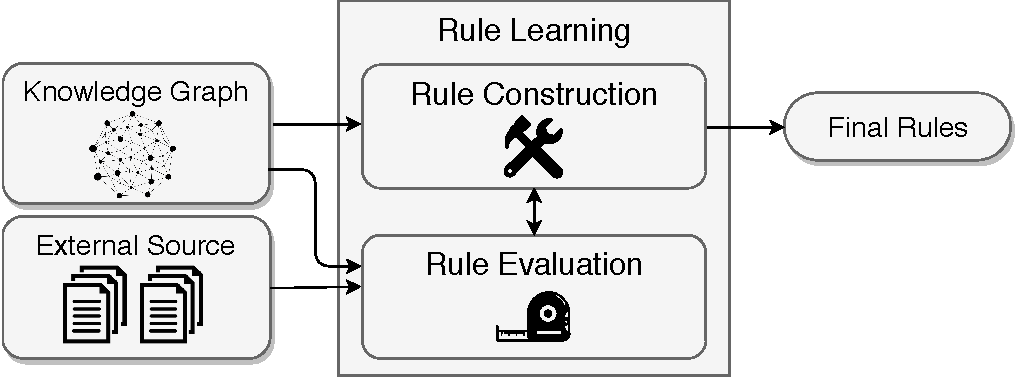
\includegraphics[width=8cm]{figures/discussion_overview}
\caption{Rule learning using external sources.}
\label{fig:discussion_overview}
\end{figure}
Toward the rule-based KG completion problem, a number of future directions could be put into consideration.
\subsubsection{Rule Learning with External Source.}
In most of rule learning systems have been proposed \cite{amie,op,rdf2rules}, while their rule construction methods may vary, the core of them is at the proposed rule evaluation metric. Various rule measures have been introduced, from the simplest to the most sophisticated one. Nevertheless, most of them are computed based on only the given graph, and cover only a small subset of local patterns in the KG, thus might wrongly estimate the quality of extracted rules since real-world KGs are usually highly incomplete.

One promising possibility to tackle this problem is to incorporate external related data from outside of the KG. The overview of such rule learning system could be described in Figure \ref{fig:discussion_overview}. The KG related external data can be extracted from many sources (e.g. crowd-sourcing, Web-extraction), and is obviously useful not only for rule evaluation, but also for rule construction over the KG. For instance, external data can give some hints about the quality of predicted facts in form of positive/negative ground truth or probability/likelihood, which could be then taken into account for rule quality evaluation or exception capturing. In addition, external KG meta-data could gives some information about the existence of certain types of facts within the KG (as exploited in CARL \cite{carl}). Moreover, we can also somehow learn rules directly from the text and then apply them back to the KG.

An alternative relational learning method for KG completion is to learn representations (i.e. embeddings) of entities and relations for predicting likelihood of unseen facts. While these methods capture global patterns in the data, and can be extended with additional unstructured knowledge (e.g., text corpus) the predictions that they produce are not interpretable. A large number of embeddings models have been proposed \cite{8047276}, in which some of them could exploit some additional text data. Hence, integrating these embedding models into the rule learning approach to deal with the mentioned issue might be a potential solution.
\subsubsection{Learning Various Rule Forms}
In KG completion problem, as mentioned, most of the rule mining approaches only mine $closed$ rules. Nevertheless, other form of rules might be also interesting. For example, rules with disjunction (e.g. $isMale(X) \vee isFemale(X) \leftarrow isPerson(X)$), rules with quantifier (e.g. $(\exists Y: playsInstrument(X, Y)) \leftarrow isMusician(X))$). These rules do not directly make predictions on the knowledge graph, because we do not know exactly which facts of the head are true. However, this kind of rules might give us some useful constraints about the knowledge graph.
